\documentclass[aspectratio=169,11pt]{beamer}
\usetheme{default}
\setbeamertemplate{navigation symbols}{}
\setbeamertemplate{footline}{%
  \hfill\insertframenumber/\inserttotalframenumber\hspace*{4pt}\vspace{2pt}%
}
\usepackage{lmodern}
\usepackage{listings}
\usepackage{tikz}
\usetikzlibrary{arrows.meta,positioning}
\usepackage{booktabs}
\usepackage{hyperref}
\usepackage{xcolor}

\definecolor{lcgreen}{HTML}{2E7D32}
\definecolor{lcblue}{HTML}{1565C0}
\definecolor{lcorange}{HTML}{EF6C00}
\definecolor{lcred}{HTML}{C62828}
\definecolor{codebg}{HTML}{F5F5F5}
\definecolor{docgray}{gray}{0.55}

\lstset{
  basicstyle=\ttfamily\scriptsize,
  backgroundcolor=\color{codebg},
  breaklines=true,
  frame=single,
  rulecolor=\color{blue!40!black},
  keywordstyle=\color{lcblue}\bfseries,
  stringstyle=\color{lcgreen},
  commentstyle=\color{docgray}\itshape,
  language=Python,
  showstringspaces=false,
  tabsize=2,
  xleftmargin=2pt,
  xrightmargin=2pt,
}

\newcommand{\docref}[1]{{\scriptsize\color{docgray}[Docs: #1]}}

\title{Output Parsing and Structured Output}
\subtitle{LangChain Section 02}
\date{March 2026 | LangChain v1.2.x}
\author{}

\begin{document}

\begin{frame}
\titlepage
\end{frame}

% ============================================================================
\begin{frame}[fragile]{The LangChain Pipeline}
\begin{center}
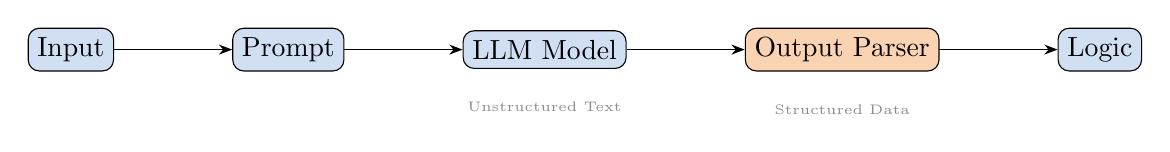
\begin{tikzpicture}[node distance=1.5cm, scale=0.85]
  \node[draw, rectangle, rounded corners, fill=lcblue!20] (input) {Input};
  \node[draw, rectangle, rounded corners, fill=lcblue!20, right=of input] (prompt) {Prompt};
  \node[draw, rectangle, rounded corners, fill=lcblue!20, right=of prompt] (model) {LLM Model};
  \node[draw, rectangle, rounded corners, fill=lcorange!30, right=of model] (parse) {Output Parser};
  \node[draw, rectangle, rounded corners, fill=lcblue!20, right=of parse] (logic) {Logic};

  \draw[-{Stealth}] (input) -- (prompt);
  \draw[-{Stealth}] (prompt) -- (model);
  \draw[-{Stealth}] (model) -- (parse);
  \draw[-{Stealth}] (parse) -- (logic);

  \node[below=0.3cm of model] {\tiny\color{docgray}Unstructured Text};
  \node[below=0.3cm of parse] {\tiny\color{docgray}Structured Data};
\end{tikzpicture}
\end{center}

\textbf{Output parsing happens after the model generates text.}
\end{frame}

\begin{frame}[fragile]{The Fundamental Problem}
\textbf{LLMs return unstructured text. Applications need structured, typed data.}

\begin{lstlisting}[language=Python]
response = llm.invoke("Extract name and age from: John is 25")
# response = "The name is John and the age is 25 years old."
# How do you get name="John" and age=25 from this string?
\end{lstlisting}

\small
\textbf{Without structured output:}
\begin{itemize}
  \item Manually parsing strings is fragile
  \item No type safety or validation
  \item Hard to integrate with downstream systems
\end{itemize}

\textbf{With structured output:}
\begin{itemize}
  \item Guaranteed schema compliance
  \item Type-safe data for your application
  \item Easier integration and testing
\end{itemize}
\end{frame}

\begin{frame}{Output Parsing Strategies}
\small
\begin{center}
\begin{tabular}{|l|p{3.5cm}|p{3.5cm}|}
\hline
\textbf{Strategy} & \textbf{Pros} & \textbf{Cons} \\
\hline
Prompting & Works everywhere & Unreliable \\
\hline
Function Calling & Very reliable & Requires support \\
\hline
JSON Mode & Good balance & Extra tokens \\
\hline
\end{tabular}
\end{center}

\docref{langchain.org/docs/modules/model\_io/output\_parsers}
\end{frame}

\begin{frame}[fragile]{StrOutputParser}
The simplest parser: extracts string content from LLM output.

\begin{lstlisting}[language=Python]
from langchain_core.output_parsers import StrOutputParser
from langchain_openai import ChatOpenAI

model = ChatOpenAI(model="gpt-4o-mini")
chain = prompt | model | StrOutputParser()

result = chain.invoke({"text": "Hello, world!"})
print(result)  # "Bonjour, le monde!"
\end{lstlisting}

\vspace{0.3cm}

\textbf{When to use:} Raw string output for summarization, translation, open-ended generation.
\end{frame}

\begin{frame}[fragile]{CommaSeparatedListOutputParser}
Parses comma-separated strings into a Python list.

\begin{lstlisting}[language=Python]
from langchain_core.output_parsers import (
    CommaSeparatedListOutputParser)

parser = CommaSeparatedListOutputParser()
prompt = ChatPromptTemplate.from_template(
    "List 5 fruits:\n{format_instructions}")

chain = prompt | model | parser
result = chain.invoke({})
# result = ["mango", "pineapple", "banana", ...]
\end{lstlisting}

\vspace{0.3cm}

\textbf{Use case:} Simple list generation with delimiter-separated values.
\end{frame}

\begin{frame}[fragile]{JsonOutputParser}
Parses JSON strings from LLM output.

\begin{lstlisting}[language=Python]
from langchain_core.output_parsers import JsonOutputParser
from pydantic import BaseModel, Field

class PersonInfo(BaseModel):
    name: str = Field(description="Full name")
    age: int = Field(description="Age in years")

parser = JsonOutputParser(pydantic_object=PersonInfo)
prompt = ChatPromptTemplate.from_template(
    "Extract person info:\n{text}\n"
    "{format_instructions}")

chain = prompt | model | parser
\end{lstlisting}

\docref{langchain.org/docs/modules/model\_io/output\_parsers/json}
\end{frame}

\begin{frame}[fragile]{PydanticOutputParser}
Combines Pydantic schema validation with output parsing.

\begin{lstlisting}[language=Python]
from langchain_core.output_parsers import PydanticOutputParser
from pydantic import BaseModel, Field

class Product(BaseModel):
    name: str = Field(..., description="Product name")
    price: float = Field(..., description="Price in USD")
    in_stock: bool = Field(default=True)

parser = PydanticOutputParser(pydantic_object=Product)
chain = prompt | model | parser
\end{lstlisting}

\vspace{0.3cm}

\docref{langchain.org/docs/modules/model\_io/output\_parsers/pydantic}
\end{frame}

\begin{frame}[fragile]{The Modern Approach: with\_structured\_output()}
ChatModels now support native structured output.

\begin{lstlisting}[language=Python]
from pydantic import BaseModel, Field
from langchain_openai import ChatOpenAI

class Sentiment(BaseModel):
    sentiment: str = Field(description="positive|negative|neutral")
    score: float = Field(description="Confidence 0-1")

model = ChatOpenAI(model="gpt-4o-mini")
structured_model = model.with_structured_output(Sentiment)

result = structured_model.invoke(
    "I love this product!")
\end{lstlisting}

\vspace{0.3cm}

\textbf{Advantages:} No explicit parser, leverages model's native capabilities, better reliability

\docref{langchain.org/docs/modules/model\_io/chat/structured\_output}
\end{frame}

\begin{frame}{with\_structured\_output() Under the Hood}
\textbf{Two Implementation Strategies}

\textbf{1. Function Calling (Preferred):}\\
Model uses function calling API to return structured data directly.

Pros: Most reliable. Cons: Requires function calling support.

\vspace{0.5cm}

\textbf{2. JSON Mode:}\\
Model constrained to output valid JSON matching schema.

Pros: Wider support. Cons: Additional prompt engineering.

\docref{langchain.org/docs/concepts/structured\_output}
\end{frame}

\begin{frame}[fragile]{Defining Schemas with Pydantic BaseModel}
Pydantic models define the expected output structure.

\begin{lstlisting}[language=Python]
from pydantic import BaseModel, Field
from typing import List, Optional

class Article(BaseModel):
    title: str = Field(..., description="Article headline")
    author: str = Field(..., description="Author name")
    tags: List[str] = Field(
        default_factory=list, description="Topic tags")
    summary: Optional[str] = Field(None)

model = ChatOpenAI(model="gpt-4o-mini")
structured_model = model.with_structured_output(Article)
\end{lstlisting}

\docref{pydantic.dev}
\end{frame}

\begin{frame}[fragile]{Complex Nested Schemas}
Output parsers handle deeply nested Pydantic structures.

\begin{lstlisting}[language=Python]
class Address(BaseModel):
    street: str
    city: str
    country: str

class Person(BaseModel):
    name: str
    age: int
    address: Address
    contact_emails: List[str]

model = ChatOpenAI(model="gpt-4o-mini")
parser = model.with_structured_output(Person)
# Full nested object automatically parsed
\end{lstlisting}
\end{frame}

\begin{frame}[fragile]{Enum Outputs and Constrained Choices}
Use enums to restrict output to specific predefined values.

\begin{lstlisting}[language=Python]
from enum import Enum

class Priority(str, Enum):
    HIGH = "high"
    MEDIUM = "medium"
    LOW = "low"

class Task(BaseModel):
    title: str
    priority: Priority
    completed: bool = Field(default=False)

model = ChatOpenAI(model="gpt-4o-mini")
parser = model.with_structured_output(Task)
# result.priority is guaranteed to be HIGH, MEDIUM, or LOW
\end{lstlisting}

\vspace{0.2cm}

\textbf{Benefit:} Enums ensure the LLM selects from allowed choices.
\end{frame}

\begin{frame}[fragile]{Optional Fields and Default Values}
Handle optional data and set sensible defaults.

\begin{lstlisting}[language=Python]
from typing import Optional, List

class Review(BaseModel):
    product_name: str
    rating: int = Field(ge=1, le=5)
    text: Optional[str] = Field(None)
    tags: List[str] = Field(default_factory=list)
    verified_purchase: bool = Field(default=False)

model = ChatOpenAI(model="gpt-4o-mini")
parser = model.with_structured_output(Review)

# Only required fields must be present
result = parser.invoke("Product: Laptop, Rating: 5")
# rating=5, text=None, tags=[], verified_purchase=False
\end{lstlisting}

\docref{pydantic.dev/docs/concepts/fields}
\end{frame}

\begin{frame}[fragile]{Custom Parsers with RunnableLambda}
Build custom parsing logic using RunnableLambda.

\begin{lstlisting}[language=Python]
from langchain_core.runnables import RunnableLambda

def parse_custom(text: str) -> dict:
    lines = text.strip().split('\n')
    result = {}
    for line in lines:
        if ':' in line:
            key, value = line.split(':', 1)
            result[key.strip()] = value.strip()
    return result

custom_parser = RunnableLambda(parse_custom)
chain = prompt | model | custom_parser
\end{lstlisting}

\vspace{0.2cm}

\textbf{Use:} Combine custom logic with LangChain for specialized parsing.
\end{frame}

\begin{frame}[fragile]{Composition: Chaining Parsers}
Combine multiple parsers for complex workflows.

\begin{lstlisting}[language=Python]
def validate_json(data: dict) -> dict:
    if data.get('age', 0) < 0:
        raise ValueError("Age cannot be negative")
    return data

json_parser = JsonOutputParser(pydantic_object=dict)
validator = RunnableLambda(validate_json)

# Chain: model to JSON parse to custom validation
chain = prompt | model | json_parser | validator
\end{lstlisting}
\end{frame}

\begin{frame}[fragile]{Error Handling: OutputParserException}
Handle parsing failures gracefully.

\begin{lstlisting}[language=Python]
from langchain_core.exceptions import OutputParserException
from pydantic import BaseModel

class Data(BaseModel):
    value: int

parser = PydanticOutputParser(pydantic_object=Data)

try:
    result = parser.parse("invalid json")
except OutputParserException as e:
    print(f"Parsing failed: {e}")
    # Handle: retry, use default, log, etc.
\end{lstlisting}

\vspace{0.3cm}

\textbf{Common Causes:}
\begin{itemize}
  \item LLM returns malformed JSON
  \item Missing required fields
  \item Type mismatch (string vs int)
  \item Enum value not in allowed set
\end{itemize}
\end{frame}

\begin{frame}[fragile]{Retry Patterns}
Automatically retry parsing with modified prompts.

\begin{lstlisting}[language=Python]
class Task(BaseModel):
    title: str
    priority: str

parser = PydanticOutputParser(pydantic_object=Task)
prompt = ChatPromptTemplate.from_template(
    "Extract task:\n{text}\n{format_instructions}\n"
    "Return ONLY valid JSON, no extra text.")

chain = (prompt | model | parser).with_fallbacks(
    [prompt | model | parser])

result = chain.invoke({"text": "Important: fix bug"})
\end{lstlisting}

\docref{langchain.org/docs/concepts/fallbacks}
\end{frame}

\begin{frame}[fragile]{Structured Retry Logic}
Implement custom retry with exponential backoff.

\begin{lstlisting}[language=Python]
import time
from langchain_core.exceptions import OutputParserException

def parse_with_retry(text, parser, max_retries=3):
    for attempt in range(max_retries):
        try:
            return parser.parse(text)
        except OutputParserException as e:
            if attempt == max_retries - 1:
                raise
            wait_time = 2 ** attempt
            time.sleep(wait_time)

result = parse_with_retry(llm_output, parser)
\end{lstlisting}
\end{frame}

\begin{frame}{Comparison: Which Parser to Use?}
\small
\begin{center}
\begin{tabular}{|l|c|c|c|}
\hline
\textbf{Parser} & \textbf{Complexity} & \textbf{Reliability} & \textbf{Speed} \\
\hline
StrOutputParser & Low & High & Very Fast \\
\hline
CommaSeparatedList & Low & Medium & Fast \\
\hline
JsonOutputParser & Medium & Medium & Medium \\
\hline
PydanticOutputParser & Medium & High & Medium \\
\hline
with\_structured\_output & Medium & Very High & Fast \\
\hline
Custom Lambda & High & Depends & Depends \\
\hline
\end{tabular}
\end{center}

\vspace{0.5cm}

\textbf{Decision Guide:}
\begin{itemize}
  \item \textbf{Just strings?} Use StrOutputParser
  \item \textbf{Typed objects?} Use with\_structured\_output
  \item \textbf{Custom logic?} Use RunnableLambda
\end{itemize}
\end{frame}

\begin{frame}{When to Use Function Calling vs JSON Mode}
\textbf{Function Calling}

Best for: Maximum reliability, strict schema enforcement

When: Model supports it (GPT-4, Claude 3+)

Trade-off: Slightly higher latency

\vspace{0.5cm}

\textbf{JSON Mode}

Best for: Balance of reliability and speed

When: Model supports JSON mode but not function calling

Trade-off: Requires explicit prompting

\vspace{0.5cm}

\textbf{Prompt plus Parsing}

Best for: Flexibility, working with any model

When: Model has no structured output support

Trade-off: Less reliable, more manual validation needed

\docref{langchain.org/docs/concepts/structured\_output}
\end{frame}

\begin{frame}{Parser Selection Guide}
\small
\begin{center}
\begin{tabular}{|l|p{8cm}|}
\hline
\textbf{Scenario} & \textbf{Recommended Parser} \\
\hline
Simple text output & StrOutputParser \\
\hline
List of items & CommaSeparatedListOutputParser \\
\hline
Typed, validated data & with\_structured\_output() \\
\hline
Custom extraction & RunnableLambda \\
\hline
Legacy Pydantic & PydanticOutputParser \\
\hline
Nested objects & with\_structured\_output() with nested Pydantic \\
\hline
Constrained choices & with\_structured\_output() with Enum \\
\hline
\end{tabular}
\end{center}
\end{frame}

\begin{frame}{Performance Considerations}
\textbf{Function Calling is Faster}
\begin{itemize}
  \item No extra prompt engineering needed
  \item Single API call with structured result
  \item Model enforces schema natively
  \item 10-20 percent lower latency than JSON mode
\end{itemize}

\vspace{0.3cm}

\textbf{Prompting Can Be Slow}
\begin{itemize}
  \item Extra tokens for format instructions
  \item May require multiple retries
  \item Additional parsing overhead
  \item Less reliable with smaller models
\end{itemize}

\vspace{0.3cm}

\textbf{Optimization:}
\begin{itemize}
  \item Use with\_structured\_output when available
  \item Cache format instructions in prompt
  \item Batch similar parsing requests
  \item Consider model choice (GPT-4o better than GPT-3.5)
\end{itemize}
\end{frame}

\begin{frame}{Token Usage and Cost}
\textbf{with\_structured\_output():}
\begin{itemize}
  \item Function calling: 50-100 extra tokens for schema
  \item JSON mode: 100-200 extra tokens for constraints
  \item Much cheaper than retry failures
\end{itemize}

\vspace{0.5cm}

\textbf{Cost Comparison (for 1000 requests):}

\begin{center}
\begin{tabular}{|l|r|}
\hline
\textbf{Approach} & \textbf{Relative Cost} \\
\hline
with\_structured\_output() & 1.0x \\
\hline
JSON Mode & 1.1x \\
\hline
Prompting plus Parsing & 1.3x (plus retries) \\
\hline
\end{tabular}
\end{center}

\vspace{0.3cm}

\textbf{Recommendation:} Use function calling when available. Cost difference is minimal but reliability gains are significant.
\end{frame}

\begin{frame}[fragile]{Quick Cheat Sheet}
\textbf{Import what you need:}
\begin{lstlisting}[language=Python]
from langchain_core.output_parsers import (
    StrOutputParser,
    JsonOutputParser,
    PydanticOutputParser,
    CommaSeparatedListOutputParser,
)
from langchain_core.runnables import RunnableLambda
from pydantic import BaseModel, Field
\end{lstlisting}

\vspace{0.3cm}

\textbf{Define your schema:}
\begin{lstlisting}[language=Python]
class MyOutput(BaseModel):
    field1: str = Field(description="...")
    field2: int = Field(ge=0, le=100)

model.with_structured_output(MyOutput)
\end{lstlisting}

\docref{langchain.org/docs/modules/model\_io/output\_parsers}
\end{frame}

\begin{frame}{Summary: Best Practices}
\begin{enumerate}
  \item \textbf{Prefer with\_structured\_output()}. Modern, reliable approach for most use cases.

  \item \textbf{Define clear Pydantic schemas}. Use Field descriptions and validators for clarity.

  \item \textbf{Handle errors gracefully}. Catch OutputParserException and implement retries.

  \item \textbf{Choose the right parser for the job}. Simple string: StrOutputParser. Typed data: with\_structured\_output.

  \item \textbf{Test with your model}. Behavior varies by model.

  \item \textbf{Monitor failure rates}. Track parsing exceptions and adjust prompts as needed.

  \item \textbf{Validate output in application}. Don't trust parser alone.
\end{enumerate}
\end{frame}

\begin{frame}{Common Gotchas}
\textbf{JSON Format Not Guaranteed}

LLMs may return malformed JSON even with instructions. Action: Always use error handling and retries.

\vspace{0.5cm}

\textbf{Enum Values Must Match Exactly}

If your Enum says HIGH, model must output HIGH. Action: Be explicit in prompts.

\vspace{0.5cm}

\textbf{Optional Fields Can Be Tricky}

Models might skip optional fields or include them as null. Action: Set explicit defaults in Pydantic.

\vspace{0.5cm}

\textbf{Large Nested Schemas Are Expensive}

Deep nesting increases token count significantly. Action: Flatten where possible, split into multiple requests.
\end{frame}

\begin{frame}{Self-Check Questions}
\begin{enumerate}
  \item What is the difference between StrOutputParser and PydanticOutputParser?

  \item When would you use with\_structured\_output() vs custom RunnableLambda?

  \item How do Enum fields help ensure valid outputs?

  \item What does OutputParserException tell you?

  \item Is function calling or JSON mode more reliable? Why?

  \item How would you handle a case where the LLM returns invalid JSON?

  \item What is the advantage of setting Field descriptions in Pydantic models?

  \item How would you validate that optional fields are handled correctly?
\end{enumerate}

\docref{langchain.org/docs/modules/model\_io/output\_parsers}
\end{frame}

\begin{frame}{Resources and Further Reading}
\begin{itemize}
  \item \textbf{LangChain Docs: Output Parsers}
    langchain.org/docs/modules/model\_io/output\_parsers

  \item \textbf{Pydantic Documentation}
    docs.pydantic.dev

  \item \textbf{Structured Outputs (Concepts)}
    langchain.org/docs/concepts/structured\_output

  \item \textbf{OpenAI Function Calling}
    platform.openai.com/docs/guides/function-calling

  \item \textbf{LangChain Source Code}
    github.com/langchain-ai/langchain
\end{itemize}

\vspace{0.5cm}

\textbf{Next in this series:} Section 03 - Prompt Engineering and Templates
\end{frame}

\begin{frame}[noframenumbering]
\begin{center}
\vspace{1.5cm}
\huge\textbf{Questions?}

\vspace{1.5cm}

\large Output parsing bridges the gap between\\
unstructured LLM output and structured application logic.

\vspace{1.5cm}

\small\textcolor{docgray}{LangChain v1.2.x | March 2026}
\end{center}
\end{frame}

\end{document}
